\documentclass[preprint,12pt]{elsarticle}
\usepackage[utf8]{inputenc}
\usepackage[T1]{fontenc}
\usepackage{lmodern}
\usepackage{amsmath,amssymb}
\usepackage{booktabs}
\usepackage{graphicx}
\usepackage{multirow}
\usepackage{xurl}
\usepackage[hidelinks]{hyperref}
\usepackage{lineno}
\journal{Journal of Systems and Software}

\begin{document}
\begin{frontmatter}

\title{Remembered, Not Generated: A Renamed-Schema Control for LLM-Provisioned Test Data, the Cost of Planning Instead of Emitting, and What Valid Data Does Not Do for LLM-Generated Tests}

\author{Vijay Prasad Javvadi\corref{cor1}}
\ead{vijay@vijayjavvadiresearch.ai}
\cortext[cor1]{Corresponding author. ORCID: 0009-0004-1192-6906.}
\address{Independent Researcher, Plainsboro, NJ, USA}

\begin{abstract}
Large language models are increasingly asked to supply test data for relational schemas. We report three executable experiments. First, we measure how close LLM-generated data comes to the fixtures that five open-source PostgreSQL schemas ship, then repeat the measurement after renaming every table and column to a synonym. Directly emitted rows match the human fixtures on the original schemas (median Jensen--Shannon distance 0.25 over the ten paired cells; 0.00 for Claude on the three widely mirrored schemas) and lose the match when the identifiers change (0.73; $p=0.016$), while their validity is unchanged ($p=1.0$) and run-to-run variation is at most 0.06: the apparent realism is recall. Second, we compare direct emission with a plan-then-execute design in which the model writes a generation plan that a constraint-aware engine executes. Neither is more valid at 500 rows per table (medians 100\,\% and 98.7\,\%), but the engine never violates a foreign key, CHECK or NOT NULL constraint, whereas emitted rows violate foreign keys and uniqueness on every schema that declares them; planning uses 29.5 times fewer tokens. Third, we inject the generated fixtures into an existing LLM test-generation pipeline with 293 frozen mutants. No fixture reliably changes the kill rate. Provisioned rows lower the share of usable generated tests, because the tests assume an empty database; a short statement of the database state in the prompt restores the yield (93\,\%) without changing the kill rate. Every input is checksummed and every number is regenerated by released scripts.
\end{abstract}

\begin{keyword}
test data generation \sep large language models \sep memorisation \sep benchmark contamination \sep referential integrity \sep mutation testing \sep empirical software engineering
\end{keyword}
\end{frontmatter}

\linenumbers

\section{Introduction}
\label{sec:intro}

A test needs data. A generated test for a service that lists orders exercises nothing unless orders exist; a fixture whose foreign keys point nowhere does not load. Developers now routinely ask a large language model (LLM) to produce test data for a schema, and the model usually obliges with rows that look plausible. This paper asks three questions about that practice and answers each with an executable experiment.

The first question is whether the plausibility is real. The schemas on which such tools are demonstrated and evaluated---Sakila, Northwind, Chinook---have been mirrored in tutorials and repositories for two decades, together with their sample data. A model that reproduces the sample data has not generated anything. We measure the fidelity of LLM-emitted rows to the shipped human fixtures of five open-source schemas, then rename every table and column to a synonym, remove the dataset names, and measure again. The difference is what recall contributed.

The second question is what a different mechanism buys. Instead of emitting rows, the model can write a compact generation plan (which generator to use per column, which distributions, which references) that a deterministic engine executes in dependency order, so that keys, uniqueness and CHECK constraints are the engine's responsibility rather than the model's. SynthData~\cite{synthdata}, the tool studied here, implements this design. We compare it with the most favourable direct-emission harness we could build, on the same schemas, scoring every emitted row by inserting it into PostgreSQL with all constraints enabled.

The third question is whether any of this matters downstream. We take an LLM test-generation pipeline with an executable mutation benchmark developed in our earlier work (manuscript under review)~\cite{javvadi2026raitg}, pre-load its database-backed services with the generated fixtures, describe those fixtures to the generator, and measure the share of usable tests and the mutation kill rate against the pipeline's own baseline. The hypothesis stated in advance was that constraint-valid data would improve both.

\paragraph{Findings.} Direct emission's fidelity to the human fixtures is largely memorisation: the categorical distance to the human data rises from a median of 0.25 to 0.73 when identifiers are renamed, far above the run-to-run variation of at most 0.06, while validity is unchanged. Plan-then-execute and direct emission reach the same validity at 500 rows per table, but for different reasons and at a thirtieth of the token cost; on declared-domain columns both arms match the human distributions, and the fidelity gap lies entirely in free-text columns, which is where recall operates. Downstream, provisioned fixtures do not raise the kill rate and reduce usable-test yield, because generated tests are written for an empty database. The advance hypothesis is rejected, the mechanism is identified, and a follow-up arm shows that stating the database state explicitly in the prompt restores the yield while leaving the kill rate where it was.

\paragraph{Contributions.}
(i) A renamed-schema control for LLM-generated relational data, with the first measurement of how much of the fidelity reported on public schemas is recall (Section~\ref{sec:rq1}).
(ii) An executable benchmark of LLM test-data provisioning against five human fixture sets, with a PostgreSQL scorer that classifies every rejected row, and the finding that validity comes from the engine, not the model (Section~\ref{sec:rq2}).
(iii) A downstream experiment showing that constraint-valid fixtures neither help nor reliably hurt an LLM test generator's kill rate and lower its usable yield, the fixture-contract mechanism behind the loss, and a follow-up arm in which an explicit database-state contract removes the loss (Section~\ref{sec:rq3}).
(iv) A defect trail for the studied engine: five defects fixed before the study version was frozen and four found by LLM-written plans afterwards, reported as results (Section~\ref{sec:defects}).

\section{Background}
\label{sec:background}

\subsection{Direct emission}
The model receives the DDL, a description of the business domain and a row target, and answers with rows. A single response cannot hold thousands of rows, so the harness requests rows in chunks, table by table in foreign-key order, and shows the model a sample of the parent keys it has already emitted so that references can be valid. This is the naive approach in its most favourable form: the model is told everything it needs to satisfy every constraint. Cost scales with the number of rows, and every row's constraints are the model's to satisfy.

\subsection{Plan-then-execute}
SynthData\footnote{\texttt{@vijaypjavvadi/synthdata}, MIT licence. The study freezes version 1.2.2; file checksums are in the artifact.} parses the DDL into tables, columns, types, primary and foreign keys, UNIQUE and CHECK constraints (including \texttt{IN} lists and enum types). It asks the model once for a YAML plan: one generator per column from a fixed vocabulary (\texttt{sequence}, \texttt{fk}, \texttt{choice} with weights, \texttt{int}, \texttt{float} and \texttt{lognormal} ranges, \texttt{date} and \texttt{datetime} ranges, \texttt{template}, \texttt{faker} methods, \texttt{expr}), with per-table row counts and a seed. It then executes the plan deterministically: tables in dependency order, foreign keys sampled from keys that exist (self-references are supported, subject to defect \#8 in Section~\ref{sec:defects}), uniqueness enforced over single and composite key sets, CHECK constraints enforced. Four profiles are available: \texttt{functional} (happy-path rows), \texttt{edge} (CHECK endpoints, maximum-length strings, NULLs in nullable columns, every enum value), \texttt{negative} (rows that each violate exactly one constraint, tagged with the violation) and \texttt{volume}. An \texttt{auto} mode infers a plan from the DDL with no LLM at all. Cost is one LLM call regardless of row count; the model controls distributions only through the plan vocabulary.

\subsection{The author's position}
SynthData is the author's tool. The study therefore gives every arm identical inputs: the same DDL, the same frozen business case, the same row targets, the same seeds. Every arm is scored with the same database and scorer. The tool version was frozen before any measured run (version 1.2.2, frozen 12 September 2026, before the first measured E1 cell). Defects found afterwards are reported as results rather than fixed, and everything is released. Section~\ref{sec:threats} returns to this.

\section{Study design}
\label{sec:method}

\subsection{Research questions}
\begin{description}
\item[RQ1 (fidelity and memorisation)] How close is LLM-provisioned data to the fixtures the projects ship, and how much of the resemblance survives when the schema's identifiers are renamed?
\item[RQ2 (validity and cost)] Does plan-then-execute produce data that satisfies the schema's declared constraints more reliably than direct emission, and at what cost?
\item[RQ3 (downstream)] Given the same LLM test generator, does provisioning constraint-valid fixtures raise the usable-test yield or the executable mutation kill rate, compared with letting the generator invent its own data?
\item[RQ4 (provider)] Do the answers hold across two model families?
\end{description}
RQ1 is answered by experiment E1 (fidelity) and its control E1b, RQ2 by E1 (validity and cost), RQ3 by E2, and RQ4 by running every LLM arm on Claude Sonnet~4.6 and GPT-4o.

\subsection{Subjects for E1 and E1b}
Table~\ref{tab:subjects} lists the five schemas. Each ships human-written sample data under an open licence and loads into PostgreSQL~16 with constraints enabled. Their shapes differ. Pagila (film rental) has 15 base tables after collapsing the payment partitions, an enum type and many-to-many bridges. Chinook (music store) has a self-referencing employee hierarchy and a composite-key bridge. Northwind (trading) has a self-reference, a composite primary key and two empty tables. \texttt{employees} (HR history) has 3.9~million rows, a CHECK constraint, a UNIQUE text column and date-range assignments. Dell DVD Store~2 (retail) has wide customer rows and no declared foreign keys between \texttt{orders}, \texttt{orderlines} and \texttt{products}. Pagila, Chinook and Northwind are widely mirrored with their sample data; \texttt{employees} is distributed with its data as a MySQL test database; Dell DVD Store~2 ships a generator rather than a fixed dataset and is the least likely of the five to have been seen with its rows. We do not know the providers' training sets, which is why the control in Section~\ref{sec:e1bdesign} exists. All five were pinned to a commit or tag and their files checksummed before any generation.

\begin{table}[t]
\centering\footnotesize\setlength{\tabcolsep}{4pt}
\caption{E1 subjects. Human rows are the shipped fixture counts; row targets for the generated arms are $\min(\text{human}, 500)$ per table.}
\label{tab:subjects}
\resizebox{\textwidth}{!}{%
\begin{tabular}{llrrl}
\toprule
Schema & Pinned source & Tables & Human rows & Notable constraints \\
\midrule
Pagila & pagila v3.1.0 & 15 & 46,273 & enum, 20 FKs \\
Chinook & chinook-database 7f67772 & 11 & 15,607 & self-ref FK, composite PK \\
Northwind & northwind\_psql cd0ef28 & 14 & 3,362 & self-ref FK, composite PK, varchar(2) \\
employees & test\_db e324b56 & 6 & 3,919,015 & CHECK, UNIQUE text, char(4) keys \\
Dell DVD Store 2 & postgresDBSamples 2bdc953 & 8 & 172,716 & no FK on order lines \\
\bottomrule
\end{tabular}}
\end{table}

\paragraph{Canonical DDL.} Each schema was exported from the PostgreSQL catalogue into one canonical file with inline PK, FK, UNIQUE, CHECK and NOT NULL clauses, enum types rewritten as \texttt{CHECK (col IN (\ldots))}, partitions collapsed and one non-portable column (Pagila's \texttt{tsvector}) dropped. Reloading the human fixtures into the canonical schema gives identical row counts and zero rejections on all five.

\paragraph{Business cases.} One text per schema, written from the project's public documentation only (never from the fixture data) and frozen with an MD5 before any run. Every arm receives the same case verbatim, plus the same row-target line.

\paragraph{Row targets.} $\min(\text{human count}, 500)$ per table, chosen after timing the direct arm at roughly 100 seconds per 100 rows. The cap is conservative against the plan arm: the direct arm's dominant failure, repeated keys across chunks, grows with the number of rows, so a higher cap would widen the validity gap in the engine's favour. Fidelity metrics compare a 500-row sample with the full human distribution.

\subsection{Arms for E1}
\begin{enumerate}
\item \textbf{Direct emission.} The model receives the canonical DDL, the business case, the table to fill, its exact row target, a sample of up to 60 already-emitted parent keys per foreign-key column, and the last 30 keys it emitted for the same table; it must answer with CSV only. Chunks of 200 rows; temperature 0; every call's tokens and latency are logged.
\item \textbf{Plan-then-execute.} SynthData's own system prompt and user-message format, temperature 0, one call; the plan is executed with seed 42 under the \texttt{functional} profile. The \texttt{edge} and \texttt{negative} profiles are executed from the run-1 plans without further LLM calls.
\item \textbf{Auto.} SynthData's no-LLM mode, seed 42.
\item \textbf{Faker.} A plain Faker~\cite{faker} script per schema with no referential resolution: what a developer gets from the ecosystem default.
\item \textbf{Human.} The shipped fixtures, unmodified.
\end{enumerate}
LLM arms run on both providers with two independent runs each: 40 LLM cells in total.

\subsection{Scoring validity}
\label{sec:scorer}
For each cell, a fresh database is created from the canonical DDL and the emitted CSVs are inserted row by row in foreign-key order inside a PL/pgSQL loop that catches every exception and records the table, row and SQLSTATE. Rows that violate anything are rejected, so a rejected parent makes its children fail their foreign key, which is the real cost of an invalid row. A retry pass re-attempts rows rejected only for foreign-key reasons until no progress is made, so that within-table order (a self-referencing hierarchy emitted child-before-parent) is never counted against an arm. Casts use base types so that declared lengths and precisions are enforced by the insert. SQLSTATE classes 23503, 23505, 23514, 23502 and 22xxx are reported as FK, UNIQUE, CHECK, NOT NULL and type/length. The scorer was validated on the human fixtures (100\,\% load on all five schemas) and on a Chinook copy with one planted violation of each class, which reports exactly the five planted rows plus their foreign-key cascade.

\subsection{Scoring fidelity}
\label{sec:fidmetrics}
Per column, against the human fixture of the same schema. Categorical columns are of two kinds. \emph{Declared-domain} columns are enum, CHECK-IN and boolean columns, whose legal values are in the DDL. \emph{Free-text} columns are text columns with at most 30 distinct human values, such as city or job title, whose values are not in the DDL. For both we compute the Jensen--Shannon distance (base~2; 0 identical, 1 disjoint) and the fraction of human values present. Numeric and date columns get the two-sample Kolmogorov--Smirnov statistic and the fraction of the human range covered; foreign-key columns the absolute difference in fan-out Gini; nullable columns the null-rate difference. Aggregates are medians over a schema's columns; surrogate keys are excluded. The declared-domain versus free-text split matters for RQ1: an arm can match a declared domain by reading the DDL, but it can match the distribution of a free-text column only by knowing the data.

\subsection{E1b: the renamed-schema control}
\label{sec:e1bdesign}
A deterministic renamer replaces every table and column identifier (54 table names and 202 distinct column names) with a synonym (\texttt{customer}$\to$\texttt{client}, \texttt{order}$\to$\texttt{purchase}, \texttt{film}$\to$\texttt{movie}, \texttt{us\_states}$\to$\texttt{state\_codes}, and so on), removes the dataset names and documentation references from the business cases, and applies the same synonyms to the case prose. Types, constraints, CHECK value lists, row targets, prompts and seeds are unchanged; the human fixtures reload into the renamed DDLs at 100\,\%, and the engine's \texttt{auto} mode reaches 100\,\% on all five. The LLM arms are rerun once per provider (20 cells) and each renamed cell is paired with the run-1 cell of the same schema, provider and arm. Two references calibrate the effect: the run-to-run variation of the original schemas (run 1 versus run 2) bounds what a rerun alone can change, and the least-mirrored schema (Dell DVD Store~2) bounds what renaming costs a model that has nothing to recall.

\subsection{E2: provisioned data downstream}
\label{sec:e2design}
E2 reuses the RAITG pipeline of~\cite{javvadi2026raitg}, whose requirements, mutants, harness and baseline run logs are archived on Zenodo as RAITG v5.0.0, with its scoring protocol unchanged. The pipeline covers 172 requirements over four community Python services (httpbin, fastapi-restful, flaskr, fastapi-task-manager). Tests are generated per requirement with the grounded prompt (SUT source injected, verification and repair on), extracted into per-service pytest harnesses, and filtered to \emph{known-good} units, those that pass on clean source. The known-good units are scored against 293 frozen mutants; a kill is a new failure or collection error. Three services have a database; httpbin has none and serves as a negative control.

For the three database-backed services we derived a DDL (flaskr's \texttt{schema.sql}; the SQLAlchemy \texttt{Task} model; the \texttt{players} table of the shipped SQLite file), wrote a business case from each project's README and REST examples, and generated fixtures with SynthData~1.2.2 (Claude plan, seed 42, three profiles). Each fixture was validated through the application itself: logins succeed and list endpoints return the fixture. The RAITG prompt (v1.5.0) gains one optional element, a \texttt{[TEST DATA]} block; without it the prompt is byte-identical to the published v1.4.0. Four arms:
\begin{description}
\item[G] the grounded arm of~\cite{javvadi2026raitg} (baseline). For Claude these are the archived run logs re-scored under the E2 harness; for GPT-4o they are new runs, since no archived GPT-4o logs exist.
\item[G+D-func] the functional fixture shown to the model and pre-loaded into the service's database at scoring.
\item[G+D-all] the same pre-loaded fixture, plus the \texttt{edge} rows shown as valid boundary payloads and the \texttt{negative} rows shown as invalid payloads with their violation tags. The database state is identical to G+D-func, so the difference isolates the information given to the model.
\item[G+D-human] the project's own fixture shown (flaskr's two users and one post; the 26 shipped players; the task manager ships none).
\item[G+D-state] added after the first four arms were scored (E2c): the G+D-func block followed by an explicit database-state contract, stating that the tables are never empty, that ids $1..N$ are taken, that the first row a test creates receives id $N+1$, that count assertions must be relative to $N$, that the listed rows are the ones to use for existing-row tests, and (for fastapi-restful) that squad numbers 1--26 are taken. The database state at scoring is identical to G+D-func; only the information given to the model differs. Run once, for Claude, against the run-1 baseline.
\end{description}
At scoring time, each arm's conftest provisions its fixture wherever the database is initialised: the default instance database, the harness fixtures, and any database a generated test creates itself through the application's \texttt{init\_db()} or \texttt{Base.metadata.create\_all()}. The promise made in the prompt therefore holds in the run. Two providers, two runs each for the first four arms. The hypothesis, written in the research plan on 11 September 2026 before any E2 run (the plan is in the artifact), was that the data block raises usable yield on the database-backed services and leaves httpbin unchanged, with any kill-rate gain concentrated on validation-path mutants. The E2c arm was designed after that hypothesis had been rejected, and its own expectations were written down before it ran (also in the artifact): that the state contract returns usable yield to the baseline level (aggregate $\ge 88$\,\%, task manager $\ge 90$\,\%), that the kill count stays within ten of the baseline, and that httpbin moves by at most seven.

\subsection{Statistics}
E1 and E1b comparisons are paired over cells (E1: schema $\times$ provider $\times$ run; E1b: renamed versus original per cell) and reported as the paired median difference with a bootstrap 95\,\% confidence interval (10,000 resamples, seed 42), Cliff's delta, and the Wilcoxon signed-rank $p$-value. Cells that share a schema are not independent, so we also report the schema-level result ($n=5$) as a sensitivity check. E2 comparisons are paired over mutants (the 293 per-mutant kill vectors of an arm versus its baseline in the same provider and run) with the exact McNemar test, a bootstrap 95\,\% confidence interval of the difference (1,000 resamples of mutants, seed 42), and a Holm correction over the twelve tests. Runs are reported side by side, never pooled.

\section{RQ1: fidelity, and what survives renaming}
\label{sec:rq1}

\subsection{Fidelity before the control}
\label{sec:fidelity}
On the surface, direct emission is far closer to the human data than plan-then-execute. Over the 18 paired cells in which both arms produced data, the median categorical Jensen--Shannon distance is 0.083 for direct emission and 1.000 for the plan arm ($p=0.003$, Cliff's $\delta=0.51$); the fraction of human categorical values reproduced is 1.00 versus 0.00 ($p=0.004$). Numeric and date distributions do not differ (KS 0.522 versus 0.501, $p=0.83$); plans cover the human numeric ranges better (0.960 versus 0.520, $p=0.019$); emitted rows imitate the human foreign-key fan-out slightly better (Gini difference 0.068 versus 0.101, $p=0.028$).

Splitting the categorical columns changes the picture. On declared-domain columns, which exist only in Pagila among the five schemas (the rating enum and two booleans; four cells), both arms match the human distributions: median JS 0.043 for the plan arm and 0.110 for direct emission. The entire categorical gap is in free-text columns (median 1.000 versus 0.083, identical to the aggregate). Two further observations point the same way. With Claude, the direct arm scores a JS distance of exactly 0.000 on 22 of the 36 categorical columns of Northwind and on 8 of the 11 of Pagila, in both runs (median 0.000): on those columns it re-emits the published dataset value for value. And on Dell DVD Store~2, the schema least likely to have been seen with its data, the direct arm's JS distance (0.41 with Claude, 0.88 with GPT-4o) and value coverage (0.88, 0.22) are no better than the plan arm's (0.47, 0.86 and 0.60, 0.19).

\subsection{The renamed-schema control}
\label{sec:e1b}
Table~\ref{tab:e1b} and Fig.~\ref{fig:e1b} pair each renamed direct-emission cell with its original run-1 cell.

\begin{table}[t]
\centering\footnotesize
\caption{E1b: direct-emission cells, original versus renamed schema (run 1). Load rate in \%; JS = median categorical Jensen--Shannon distance to the human data; cov = fraction of human categorical values reproduced; $\Delta$JS = renamed $-$ original.}
\label{tab:e1b}
\resizebox{\textwidth}{!}{%
\begin{tabular}{llccccccc}
\toprule
Schema & Provider & load orig & load ren & JS orig & JS ren & $\Delta$JS & cov orig & cov ren \\
\midrule
Chinook & Claude & 93.8 & 99.2 & 0.000 & 0.326 & $+0.33$ & 1.00 & 0.80 \\
Chinook & GPT-4o & 99.7 & 99.7 & 1.000 & 1.000 & $0.00$ & 0.00 & 0.00 \\
Northwind & Claude & 98.4 & 97.2 & 0.000 & 0.263 & $+0.26$ & 1.00 & 0.95 \\
Northwind & GPT-4o & 77.3 & 87.8 & 0.587 & 1.000 & $+0.41$ & 0.63 & 0.00 \\
Pagila & Claude & 99.9 & 99.6 & 0.000 & 1.000 & $+1.00$ & 1.00 & 0.00 \\
Pagila & GPT-4o & 94.7 & 96.1 & 1.000 & 1.000 & $0.00$ & 0.00 & 0.00 \\
employees & Claude & 99.8 & 95.4 & 0.054 & 0.085 & $+0.03$ & 1.00 & 1.00 \\
employees & GPT-4o & 98.6 & 98.7 & 0.083 & 0.389 & $+0.31$ & 1.00 & 1.00 \\
Dell DVD Store 2 & Claude & 100 & 97.7 & 0.406 & 0.589 & $+0.18$ & 0.88 & 0.83 \\
Dell DVD Store 2 & GPT-4o & 100 & 100 & 0.875 & 0.875 & $0.00$ & 0.22 & 0.22 \\
\midrule
median & & 99.2 & 98.2 & 0.245 & 0.732 & $+0.22$ & 0.94 & 0.51 \\
\bottomrule
\end{tabular}}
\end{table}

\begin{figure}[t]
\centering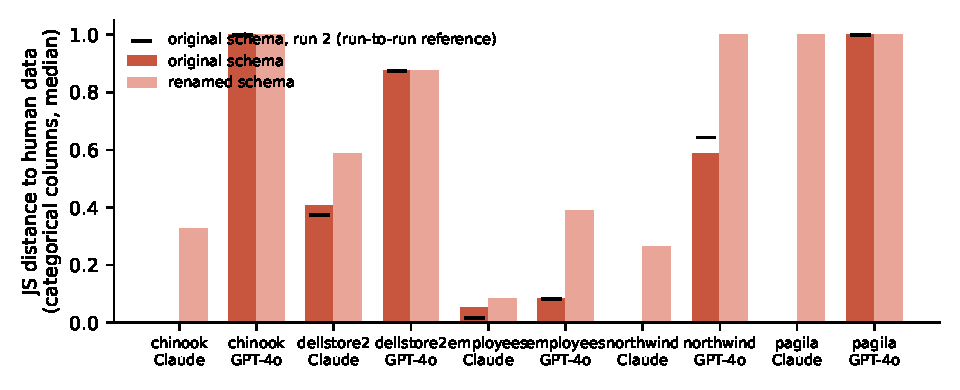
\includegraphics[width=\textwidth]{figures/fig3_e1b_memorisation}
\caption{E1b: categorical distance of directly emitted data to the human fixtures, original versus renamed identifiers (direct arm, run 1). The black tick on each original bar is the same cell's run-2 value, i.e.\ the run-to-run reference (median $|\Delta|$ 0.000, maximum 0.056). Claude's exact reproduction of Northwind, Chinook and Pagila disappears when the names change; Dell DVD Store~2, the least-mirrored schema, moves by 0.18 (Claude) and 0.00 (GPT-4o).}
\label{fig:e1b}
\end{figure}

\paragraph{Validity is unaffected.} Direct-emission load rates do not change under renaming (median 99.2\,\% versus 98.2\,\%; paired median difference 0.000, 95\,\% CI $[-0.012, +0.028]$; $p=1.0$). The models' ability to satisfy constraints does not depend on recognising the dataset, which also rules out the alternative reading that the renamed schemas are simply harder to understand.

\paragraph{The fidelity advantage does not survive.} The direct arm's median categorical JS distance rises from 0.245 to 0.732 (paired median difference $+0.22$, 95\,\% CI $[0.00, +0.36]$; $p=0.016$), its value coverage falls from 0.94 to 0.51 ($p=0.062$), and its numeric/date KS statistic rises from 0.522 to 0.602 (median difference $+0.06$, CI $[0.00, +0.09]$; $p=0.023$). Two references put these deltas in scale. The run-to-run variation of the same metric on the original schemas (run 1 versus run 2, ten schema--provider pairs) has median 0.000 and maximum 0.056, so a rerun alone does not move the distance. And on Dell DVD Store~2, the least-mirrored schema, renaming costs Claude 0.18 and GPT-4o 0.00, which bounds what synonyms cost a model with nothing to recall. On the three widely mirrored schemas Claude's deltas are $+0.33$ (Chinook), $+0.26$ (Northwind) and $+1.00$ (Pagila), and GPT-4o, which was already at JS~1.0 on Chinook and Pagila, moves $+0.41$ on Northwind, the one it had partly reproduced. Claude's exact reproduction of Pagila (JS 0.000, coverage 1.0) becomes a disjoint distribution (JS 1.000, coverage 0.0).

We read this as memorisation, with the stated caveats: the effect is far above run-to-run noise and above the renaming cost on the unfamiliar schema, and it appears where the published data is famous and the model had reproduced it exactly. Under renamed schemas the direct arm's categorical fidelity (median 0.73) is much closer to the plan arm's (median 1.0) than the 0.08-versus-1.00 comparison of Section~\ref{sec:fidelity} suggested. The RQ1 answer is therefore: on an unseen schema neither approach reproduces the categorical distributions of the human data; the plan arm covers numeric ranges better; the direct arm imitates fan-out slightly better; and the large categorical advantage of direct emission on public schemas is recall of Northwind, Sakila and Chinook.

One cue survives renaming. Claude's renamed-Pagila plan still placed rental dates in 2005--2006, the Sakila era, so structural recognition is not fully removed by identifier renaming. The control removes lexical identity, not structure; a stronger control would perturb values as well, or use a schema published after the providers' training cut-offs.

\paragraph{The plan arm under renaming.} Plan-arm load falls from a mean of 0.888 (run 1) to 0.711, and every sub-100 renamed cell is again defect \#6 or \#7 (Section~\ref{sec:defects}): with synonym names both models reached for \texttt{expr} date arithmetic in 4 of 10 plans (3 of 20 in E1), and the engine handles it wrongly. The plan arm's validity ceiling is set by the engine's handling of LLM-written plans, not by the model.

\section{RQ2: validity and cost}
\label{sec:rq2}

\subsection{Validity}
Table~\ref{tab:e1load} and Fig.~\ref{fig:e1load} give the load rate of every cell. Over the 20 paired (schema, provider, run) cells the plan arm's mean is 0.886 with median 1.000 and the direct arm's mean is 0.962 with median 0.987. The two engine aborts (defect \#6, Northwind with GPT-4o, both runs), counted as zero, put the direct arm ahead on the mean by 0.076; on the paired median difference the arms are level ($+0.004$, 95\,\% CI $[-0.017, +0.015]$; Wilcoxon $p=0.85$; schema-level $p=0.81$). Excluding the two aborts ($n=18$) the means are 0.985 and 0.983 and the plan arm is marginally ahead (paired median difference $+0.006$, CI $[+0.002, +0.017]$; Cliff's $\delta=0.53$; $p=0.29$). We state the result as: at 500 rows per table on these schemas, plan-then-execute has no validity advantage over direct emission, and a user who counts the aborts sees it slightly behind. The difference between the arms is in how they fail.

\begin{table}[t]
\centering\footnotesize\setlength{\tabcolsep}{3.5pt}
\caption{E1 load rate (\% of emitted rows accepted by PostgreSQL with all constraints on), run 1 / run 2. ``abort'' = the engine aborted on the LLM-written plan (defect \#6) and produced no data, counted as 0.}
\label{tab:e1load}
\resizebox{\textwidth}{!}{%
\begin{tabular}{lcccccccc}
\toprule
& \multicolumn{2}{c}{plan-then-execute} & \multicolumn{2}{c}{direct emission} & auto & Faker & human \\
\cmidrule(lr){2-3}\cmidrule(lr){4-5}
Schema & Claude & GPT-4o & Claude & GPT-4o & (no LLM) & & \\
\midrule
Chinook   & 100 / 100 & 100 / 100 & 93.8 / 98.1 & 99.7 / 99.6 & 100 & 99.3 & 100 \\
Northwind & 100 / 100 & abort / abort & 98.4 / 97.7 & 77.3 / 77.1 & 100 & 23.5 & 100 \\
Dell DVD Store 2 & 93.8 / 100 & 93.9 / 93.8 & 99.97 / 98.8 & 100 / 99.97 & 100 & 100 & 100 \\
Pagila    & 100 / 100 & 100 / 90.8 & 99.9 / 99.6 & 94.7 / 94.4 & 100 & 52.3 & 100 \\
employees & 100 / 100 & 100 / 100 & 99.8 / 99.3 & 98.6 / 97.7 & 100 & 0.4 & 100 \\
\bottomrule
\end{tabular}}
\end{table}

\begin{figure}[t]
\centering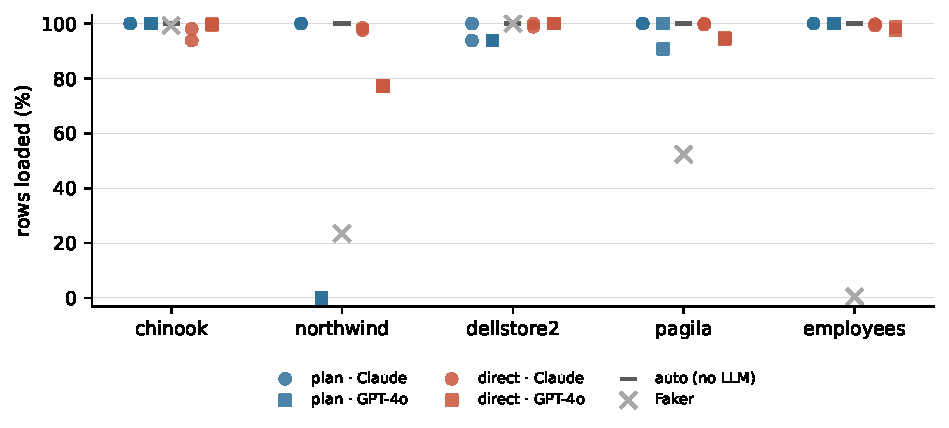
\includegraphics[width=\textwidth]{figures/fig1_e1_load}
\caption{E1 load rate per schema and arm (both providers, both runs). The plan arm is at 100\,\% except where an engine defect bites; direct emission degrades with schema difficulty and model.}
\label{fig:e1load}
\end{figure}

The plan arm is bimodal: 14 of the 18 executed cells load at exactly 100\,\%, and each of the remaining four is attributable to one engine defect visible in the plan and the rejection log. Three Dell DVD Store~2 cells lose 185--187 rows to duplicate primary keys because the model wrote \texttt{\{gen: fk, ref: inventory.prod\_id\}} for a primary-key column and the engine sampled the reference with replacement (defect \#7; the schema declares no foreign key there, which is why the model reached for one). One Pagila cell loses 443 rows because an \texttt{expr} generator received its date operand as a string and concatenated instead of adding (\texttt{2025-03-18 16:25:007}; defect \#6), and the two Northwind GPT-4o cells abort on the same defect. Across all executed plan cells the engine emitted zero foreign-key, CHECK and NOT NULL violations; its 559 UNIQUE and 443 type rejections are the two defects.

Direct emission is never 100\,\% on a schema with declared foreign keys (its one 100\,\% is Dell DVD Store~2, which declares none), and its rejections are the model's: 504 foreign-key, 1,009 uniqueness, 4 NOT NULL and 79 type/length violations over 20 cells. The effect grows with schema difficulty and shrinks with model strength: on Northwind, GPT-4o loads 77.3 and 77.1\,\% in the two runs (152/139 foreign-key, 147/164 uniqueness and 13/12 type rejections), Claude 98.4 and 97.7\,\%. Repeated keys across chunks are the dominant failure: the model is told the last 30 keys it emitted and still repeats keys from earlier chunks.

The baselines frame the result. The engine's no-LLM \texttt{auto} mode loads 100\,\% on all five schemas. Validity, on these schemas, comes from the engine; the LLM's contribution to the plan arm is the plan's semantics, which Section~\ref{sec:rq1} measures as fidelity. The Faker script, the ecosystem default, loads 100\,\% only where every foreign key happens to point at a table whose keys are $1\ldots N$ (Dell DVD Store~2, Chinook) and collapses elsewhere (Northwind 23.5\,\%, Pagila 52.3\,\%, \texttt{employees} 0.4\,\%): the referential engine is what a Faker script lacks.

\paragraph{Profiles.} Both were executed from the run-1 plans without further LLM calls. The \texttt{edge} profile loads at 100\,\% on every schema except Dell DVD Store~2 (93.8\,\%, defect \#7 again). The \texttt{negative} profile loads at 0\,\% on every schema, which is the property a negative fixture must have: each of its rows is rejected for a stated class (type, NOT NULL, foreign key or CHECK) that the scorer reports.

\subsection{Cost}
Per cell (Fig.~\ref{fig:e1tokens}), the plan arm uses a median of 3,472 tokens in one call and the direct arm 90,340 tokens in 14--45 calls; the median of the per-cell ratios is 29.5 (the ratio of the medians is 26.0). Wall-time medians are 15\,s and 658\,s (per-cell median ratio 46; the longest direct cell, Pagila with Claude, took 28 minutes). Over the study the plan arm consumed 40k input and 31k output tokens, the direct arm 865k and 1,441k.

\begin{figure}[t]
\centering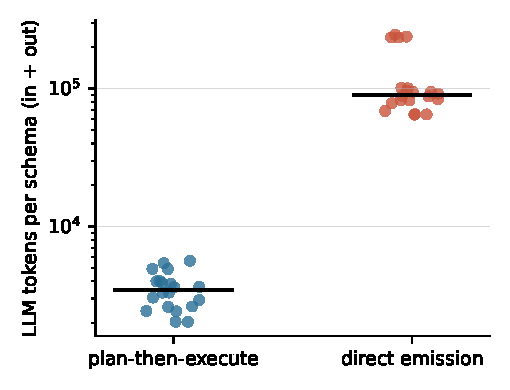
\includegraphics[width=0.5\textwidth]{figures/fig2_e1_tokens}
\caption{LLM tokens per schema cell (in + out, log scale; bars are medians): 3,472 for plan-then-execute versus 90,340 for direct emission.}
\label{fig:e1tokens}
\end{figure}

\section{RQ3: provisioned data and LLM-generated tests}
\label{sec:rq3}

\subsection{Harness}
Two harness issues surfaced during scoring and were fixed before any number was final; both are recorded because the second changes a baseline. First, the fixture's password hashing (werkzeug's default 260k PBKDF2 rounds, re-run before every test and on every \texttt{init\_db()} call) pushed the flaskr suite past the scorer's 90-second limit, which the RAITG protocol counts as a kill. Hashes are therefore memoised with a low iteration count; logins are unaffected, since the verifier reads the method from the stored hash. Second, one GPT-4o flaskr unit calls the application's \texttt{init\_db\_command()} at module level. The resulting \texttt{SystemExit} inside pytest's collection aborted every pytest process for that service. The original group-level known-good filter could not attribute the failure to a unit and kept all 130, and the scorer then saw the same exit status on the baseline and on every mutant, that is, zero kills. The E2 harness therefore adds a per-unit pre-screen before the known-good filter: each unit runs alone under a 30-second wall cap (the limit the RAITG protocol already applies per test function, which pytest's timeout cannot apply to module-level code), and units that cannot pass alone are excluded and recorded. The pre-screen removes units; it cannot add kills. Every arm, including the baseline for both providers, was re-scored under this one harness before any comparison was made. The Claude baseline logs re-scored under it give 161 and 169 kills against the archived 160 and 159; the difference is three fastapi-restful units that pass only after an earlier unit has warmed the service's ten-minute response cache, order-dependent units that the stricter filter removes. No E2 chunk contains a timeout-based kill.

\subsection{Usable yield and kill rate}
Table~\ref{tab:e2} and Figs.~\ref{fig:e2kills}--\ref{fig:e2yield} give the aggregate results; Table~\ref{tab:e2pair} the paired statistics.

\begin{table}[t]
\centering\footnotesize\setlength{\tabcolsep}{4pt}
\caption{E2: mutants killed (of 293) and usable yield (known-good units / emitted units) per arm, provider and run.}
\label{tab:e2}
\begin{tabular}{lcccc}
\toprule
Arm & Claude r1 & Claude r2 & GPT-4o r1 & GPT-4o r2 \\
\midrule
G (grounded RAITG) & 161 (88\,\%) & 169 (89\,\%) & 106 (52\,\%) & 109 (59\,\%) \\
G + SynthData functional fixture & 158 (85\,\%) & 167 (84\,\%) & 115 (53\,\%) & 109 (49\,\%) \\
G + functional + edge/neg.\ payloads & 170 (83\,\%) & 167 (85\,\%) & 106 (50\,\%) & 113 (48\,\%) \\
G + project's own fixture & 145 (87\,\%) & 167 (81\,\%) & 109 (51\,\%) & 102 (48\,\%) \\
G + functional fixture + state contract (E2c) & 160 (93\,\%) & --- & --- & --- \\
\bottomrule
\end{tabular}
\end{table}

\begin{table}[t]
\centering\footnotesize
\caption{E2 paired versus G, same provider and run: difference in mutants killed, McNemar exact $p$, Holm-adjusted $p$ over the twelve pre-planned tests, bootstrap 95\,\% CI. The E2c arm was tested afterwards and is reported unadjusted.}
\label{tab:e2pair}
\resizebox{\textwidth}{!}{%
\begin{tabular}{llrrrrrr}
\toprule
Provider & Arm & r1 $\Delta$ & $p$ & $p_{\text{Holm}}$ & CI & r2 $\Delta$ ($p$) & CI \\
\midrule
Claude & functional & $-3$ & 0.51 & 1.0 & $[-9,+3]$ & $-2$ (0.75) & $[-8,+4]$ \\
Claude & func + edge/neg & $+9$ & 0.022 & 0.25 & $[+2,+16]$ & $-2$ (0.73) & $[-7,+3]$ \\
Claude & project fixture & $-16$ & $<$0.001 & 0.005 & $[-25,-8]$ & $-2$ (0.82) & $[-11,+6]$ \\
Claude & func + state contract (E2c) & $-1$ & 1.0 & --- & $[-6,+3]$ & --- & --- \\
GPT-4o & functional & $+9$ & 0.19 & 1.0 & $[-2,+22]$ & $0$ (1.0) & $[-9,+11]$ \\
GPT-4o & func + edge/neg & $0$ & 1.0 & 1.0 & $[-12,+11]$ & $+4$ (0.57) & $[-6,+14]$ \\
GPT-4o & project fixture & $+3$ & 0.63 & 1.0 & $[-5,+11]$ & $-7$ (0.19) & $[-16,+1]$ \\
\bottomrule
\end{tabular}}
\end{table}

\begin{figure}[t]
\centering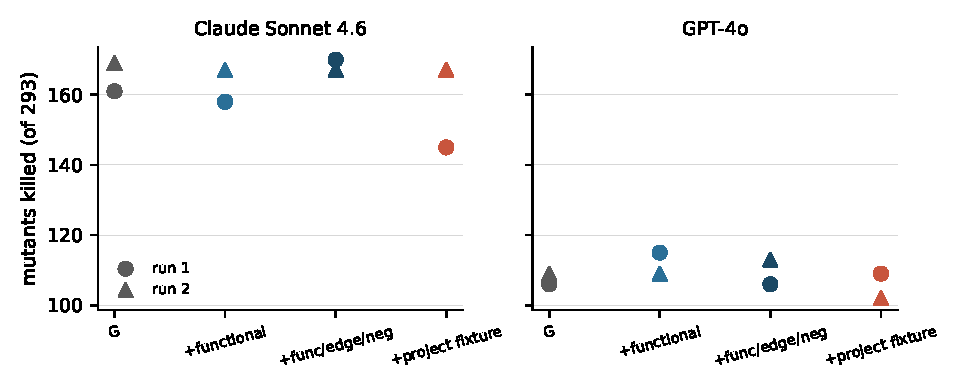
\includegraphics[width=\textwidth]{figures/fig4_e2_kills}
\caption{E2: mutants killed per arm (circles run 1, triangles run 2). No arm moves the kill rate reliably.}
\label{fig:e2kills}
\end{figure}

\begin{figure}[t]
\centering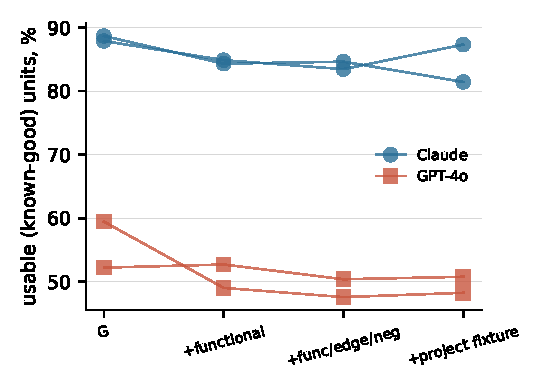
\includegraphics[width=0.55\textwidth]{figures/fig5_e2_yield}
\caption{E2: usable yield per arm. Provisioned fixtures lower the share of generated tests that pass on clean source for Claude.}
\label{fig:e2yield}
\end{figure}

\paragraph{The advance hypothesis is rejected.} A provisioned fixture does not raise usable yield. For Claude it lowers it, from 88--89\,\% to 83--85\,\%, and most on the task manager (known-good units 241 of 254 in G, 176 of 275 with the functional fixture). The failing units explain why: with 20 tasks pre-loaded, generated tests that create one task and assert a count of one, or that assume the row they created has id~1, fail on clean source, even though the prompt lists the pre-loaded rows and their ids. Provisioned rows conflict with the empty-database assumption the generator carries, and listing the rows does not remove the conflict.

\paragraph{Stating the contract does (E2c).} The G+D-state arm adds to the same functional block an explicit statement of what the pre-loaded rows imply for a test: ids $1..N$ are taken, a created row receives $N+1$, counts are relative to $N$. With the database state unchanged, usable yield returns to and slightly above the baseline: 1,207 of 1,294 units (93.3\,\%) against 87.9\,\% for G and 84.9\,\% for G+D-func, and on the task manager 271 of 281 (96.4\,\%) against 241 of 254 (94.9\,\%) and 176 of 275 (64.0\,\%). The generated tests read the contract: the failing patterns of G+D-func (assert a count of one; assume id~1) are replaced by tests that capture the id from the create response and assert relative counts or the presence of the row they created. The kill count is 160 against the baseline's 161 (paired difference $-1$; 2 arm-only and 3 baseline-only mutants; McNemar $p=1.0$; bootstrap CI $[-6,+3]$), with httpbin at $+1$, fastapi-restful and flaskr unchanged, and the task manager at 36 against 38 (32 with the functional block alone). All three expectations written down before the run hold. The block costs 16\,\% more input tokens than G (1.44M against 1.24M), about the same as the functional block alone. The yield loss of provisioning is therefore a fixture-contract problem that the prompt can solve; solving it does not change what the tests detect.

\paragraph{No arm reliably changes the kill rate.} Of twelve paired comparisons, two are nominally significant and neither replicates. Claude with the boundary/negative payloads gains 9 mutants in run 1 ($p=0.022$; Holm-adjusted $p=0.25$), driven by fastapi-restful (16$\to$25), the validation-path mutants (409 on a duplicate squad number, 422 on an invalid payload) that the advance hypothesis named; in run 2 the baseline itself kills 25 on that service and the arm adds nothing. Claude with the project's fixture loses 16 in run 1 ($p<0.001$; Holm-adjusted $p=0.005$), a flaskr collapse (31$\to$15, with 113 of 163 units usable) that does not recur in run 2 (21). A 9-mutant change is 3 percentage points of the 293. GPT-4o's differences are within $\pm 9$ with 17--37 discordant mutants per comparison. The minimum difference the exact test can detect at these discordant counts is roughly 6--12 mutants, and the run-to-run variation of the baseline itself is of that size (161 versus 169 for Claude). httpbin, the service with no database and no block, moves by at most seven mutants (between $+1$ and $+7$ for Claude, between $-5$ and $+2$ for GPT-4o), inside the run-to-run band, as a control should. Two runs are not enough to separate a ten-mutant arm effect from run-to-run variation on this harness, and we report both runs rather than the favourable one.

\paragraph{Provider (RQ4).} GPT-4o is a different regime: about three tests per requirement (516 units per run against Claude's 1,300), half of them unusable, three to five times more repair passes, and 102--115 kills whatever the arm. The RAITG prompt was developed against Claude, so the two providers are not compared as equals; RQ4 is answered as ``the null replicates'', not ``the providers are equivalent''.

\paragraph{Cost.} The functional block adds 14\,\% input tokens per condition run (Claude 1.24M$\to$1.41M), the functional block with the state contract 16\,\% (1.44M), the full block 40\,\% (1.74M); output tokens change by less than 10\,\% and repair counts do not rise.

\section{The defect trail}
\label{sec:defects}
An executable study against a tool finds defects in the tool. We fixed the ones found before the study version was frozen and report the ones found afterwards as results. Five were found and fixed before freezing at 1.2.2. Numeric$(p,s)$ precision was ignored (Pagila \texttt{rental\_rate} received 752.09; 199 of 200 film rows were rejected, with a cascade into four child tables). A composite \texttt{PRIMARY KEY} was not treated as a uniqueness set (305 duplicate bridge rows on Chinook). A UNIQUE text column with a small fake-value pool aborted generation. \texttt{varchar(n)} was not enforced for plan-driven generators (a three-character state abbreviation went into \texttt{varchar(2)}). And \texttt{\{gen: fk\}} on a column without a declared foreign key aborted the run. The v1.1.0 smoke numbers that motivated these fixes (Pagila 60.1\,\%, \texttt{employees} aborting) are in the artifact's cell table. Four were found after freezing, by LLM-written plans. \#6: \texttt{expr} receives dates as strings (seven cells across E1 and E1b). \#7: \texttt{fk} on a primary-key column samples with replacement (E1 and E1b, Dell DVD Store~2). \#8: a self-referencing \texttt{fk} on a NOT NULL column emits NULL for the first rows (found while validating the E2 fixtures; no E1 cell is affected). \#9: the YAML parser rejects a multi-line flow sequence that PyYAML accepts (the E2 task-manager plan, twice at temperature 0; re-serialised mechanically for the fixture and recorded). Every plan-arm miss in E1 and E1b is \#6 or \#7. The plan arm's validity ceiling is the engine's plan handling, and a user of version 1.2.2 inherits these defects.

\section{Threats to validity}
\label{sec:threats}
\paragraph{Construct.} Validity is measured as acceptance by PostgreSQL with declared constraints; undeclared business rules (an order line for a discontinued product) are invisible to it, and the human schemas declare almost no CHECK constraints, so the constraint surface is dominated by keys and nullability. Fidelity metrics are column-wise and blind to cross-column coherence (a player whose position and abbreviation disagree, as SynthData's E2 fixtures do); the fixture arms in E2 test provisioning, not realism, and the project-fixture arm is the realism control. Free-text fidelity can only be achieved by knowing the data, which is why we report declared-domain and free-text columns separately. In E2, a kill is a failing or crashing unit; script-style units bypass pytest's per-test timeout, which is why the pre-screen exists.
\paragraph{Internal.} The direct arm is the most favourable naive design we could build (parent keys shown, chunked, resumable); a weaker one would only widen the gap. The 500-row cap favours direct emission (Section~\ref{sec:method}). Temperature 0 is not determinism: the same prompt produced plans that parsed and plans that did not, and run-to-run differences of ten mutants. The harness hardening in E2 was applied uniformly after discovery, and both scorings of the Claude baseline are on record. The E2 fixture's flaskr passwords are stored with a low PBKDF2 iteration count for timing reasons; login semantics are unchanged.
\paragraph{Conclusion.} E1 has 20 cells over five schemas and E1b ten pairs; cells sharing a schema are not independent, and the schema-level test ($n=5$) is reported alongside. E2's two runs give a minimum detectable effect of 6--12 mutants, the size of the baseline's own run-to-run variation. Twelve E2 tests are Holm-corrected; the E2c arm is a single run added afterwards, tested against expectations written before it ran, and reported unadjusted.
\paragraph{External.} Five schemas, four services, two providers, 500 rows per table. Memorisation is only partly controlled: renaming removes lexical cues, not structural ones (Section~\ref{sec:e1b}). GPT-4o's low unit yield confounds the provider comparison in E2. The E2 baseline is asymmetric (published Claude logs, fresh GPT-4o runs).
\paragraph{Conflict of interest.} The tool is the author's. The mitigations are identical inputs and scoring for every arm, a version frozen before the first measured run, an independent no-LLM and a Faker baseline, published defects, and a released artifact that regenerates every number. The paper's central claims are that validity comes from the engine rather than the model, that the fidelity advantage belongs to the competing approach and is recall, and that the downstream hypothesis is rejected; none of these favours the tool.

\section{Related work}
\label{sec:related}

\paragraph{LLMs as test-data generators.} Baudry et al.~\cite{baudry2024generators} asked LLMs either to emit test data directly or to write test-data generator code, across languages and cultural contexts, and evaluated domain adequacy and executability; their generator-writing mode is the nearest precedent for plan-then-execute, and their evaluation did not check relational constraints or compare against human fixtures. Kannan et al.~\cite{kannan2025sqltestdata} generated test data for complex SQL schemas with an LLM in a privacy-restricted industrial setting and judged structural and semantic validity with schema checks and an LLM-as-a-judge; our scorer replaces the judge with the database. Neither study controlled for the possibility that the model had seen the data. Deep generative models for tabular data, from conditional GANs~\cite{xu2019ctgan} to fine-tuned language models that serialise rows as text~\cite{borisov2023great}, target distributional fidelity for machine-learning use. Our consumer is a test, so hard constraints are the primary requirement. And our data is requested for a public schema rather than sampled from a private table, which is what raises the recall question.

\paragraph{Test data for database applications.} AGENDA~\cite{chays2004agenda} populated databases from schema constraints and user-supplied value sets; later work generated databases to satisfy declarative constraints and cardinality targets~\cite{arasu2011declarative}, produced realistic values at scale for benchmarking~\cite{bruno2005flexible,houkjaer2006simple}, derived inputs from the queries a program issues~\cite{emmi2007dynamic}, and defined coverage criteria over SQL predicates~\cite{tuya2010full}. Search-based generation of test data for a schema's integrity constraints~\cite{kapfhammer2013search,mcminn2015effectiveness} is the closest ancestor of the engine studied here; SynthData's \texttt{negative} profile is a generator-vocabulary rendering of that idea, and our scorer is the oracle those works rely on. None of this literature considered a language model as the author of the generator.

\paragraph{Memorisation and contamination.} That language models reproduce training data verbatim is established~\cite{carlini2021extracting}, and benchmark contamination is a recognised problem in natural-language evaluation~\cite{magar2022contamination,sainz2023contamination}. For code, ReCode~\cite{wang2023recode} evaluates generation models under semantics-preserving perturbations, including identifier renaming; the renamed-schema control is the same idea applied to relational fixtures, whose value is precisely that they are public and long-lived, so held-out data is not available. Its result---a fidelity advantage that disappears under renaming while validity does not move---is the relational counterpart of the contamination effects reported for text benchmarks, and we are not aware of a prior measurement of it for LLM-generated test data.

\paragraph{LLM-generated tests and their execution.} LLM unit-test generation has been evaluated on coverage and correctness~\cite{schafer2024testpilot,siddiq2024junit,yuan2024chattester}, compared with search-based generation~\cite{tang2024chatgptsbst} and combined with it~\cite{lemieux2023codamosa}; surveys~\cite{wang2024survey} catalogue the design space. Where these studies evaluate against mutated programs they inherit mutation analysis and its caveats about mutant validity~\cite{just2014mutants,papadakis2019mutation}; E2 reuses an existing, archived executable benchmark so that the only variable is the data block. Two findings anticipate ours: generated tests often fail for environmental reasons, such as wrong fixtures and assumptions about state~\cite{schafer2024testpilot,yuan2024chattester}, and the test-pattern literature distinguishes fresh fixtures built by each test from shared or prebuilt fixtures that tests must respect~\cite{meszaros2007xunit}. LLM-generated tests, in our data, behave as if every fixture were fresh.

\paragraph{Faker.} The de facto tool for test data in Python is Faker~\cite{faker}, which produces plausible scalar values with no notion of a schema; our Faker arm is that default applied per table, and its foreign-key failures on four of five schemas quantify what a relational engine adds before any LLM is involved.

\section{Conclusion}
\label{sec:conclusion}
The realism that LLM-emitted test data shows on well-known schemas is largely recall of the published fixtures: it disappears when the identifiers are renamed, while the model's ability to satisfy the schema's constraints does not change. Evaluations of LLM data generation on public schemas therefore need a renamed-schema control, and we provide one. Planning instead of emitting does not buy validity at 500 rows per table; the engine's guarantees hold by construction and its misses are engine defects, the model's misses are foreign-key and uniqueness violations that grow with schema difficulty, and planning costs a thirtieth of the tokens. Constraint-valid fixtures do not make an LLM test generator kill more mutants, and they reduce the share of usable tests because the generator writes for an empty database. Telling the generator which identifiers are taken and that counts start at $N$ restores the yield without changing the kill rate. A provisioning tool should therefore ship a fixture together with its state contract, and a test generator should expect one.

\section*{Data availability}
The complete artifact (pinned subjects with checksums, canonical and renamed DDLs with rename maps, frozen business cases, row targets, the E2 DDLs, cases, fixtures and prompt blocks, every arm's output with per-call tokens and latency, every score and metric file, the per-mutant kill vectors, known-good lists and pre-screen records of E2, the scoring harness, the cell-table builder and the scripts that regenerate every table, figure and statistic in this paper) is archived on Zenodo as \texttt{paperH-artifact} v1.1.0, DOI \href{https://doi.org/10.5281/zenodo.22939052}{10.5281/zenodo.22939052}, and mirrored at \href{https://github.com/javvadivijayprasad/llm-testdata-memorisation}{github.com/javvadivijayprasad/llm-testdata-memorisation} (tag \texttt{v1.1.0}, the same files). SynthData~1.2.2 is published on npm; its file checksums are in the artifact.

\section*{CRediT authorship contribution statement}
Vijay Prasad Javvadi: Conceptualization, Methodology, Software, Validation, Formal analysis, Investigation, Data curation, Writing -- original draft, Writing -- review \& editing, Visualization.

\section*{Declaration of competing interest}
The author is the developer of SynthData. See Section~\ref{sec:threats}.

\section*{Declaration of generative AI use}
Generative AI (Claude) was used as a coding and drafting assistant under the author's direction; the author takes full responsibility for the content. All LLM calls that are part of the experiments are described in the paper and logged in the artifact.

\bibliographystyle{elsarticle-num}
\bibliography{references}
\end{document}
